\documentclass[
print,
  11pt,
  table,   
  nolof,    
  nolot,
  oneside,
  draft
]{fithesis3}

\usepackage[resetfonts]{cmap}
\usepackage[main=czech,english]{babel}       
%% The following section sets up the metadata of the thesis.

\thesissetup{
    university    = mu,
    faculty       = fi,
    type          = mgr,
    author        = Bc. Milan Valúšek,
    gender        =m,
    advisor       = prof. RNDr. Jiří Hřebíček\, CSc.,
    title         = {Podpora výuky matematiky v LMS Moodle s využitím Maple T.A.},
    TeXtitle      = {Podpora výuky matematiky v LMS Moodle s využitím Maple T.A.},
    keywords      = {E-learning, Learning Management system, Learning Tools Interoperability, Moodle, Maple T.A., webové služby, integrace },
    TeXkeywords   = {E-learning, Learning Management system, Learning Tools Interoperability, Moodle, Maple T.A., webové služby, integrace },
}
\thesislong{abstract}{
Práce se zabývá e-learningovými systémy LMS Moodle a Maple T.A., jejich základním stavebním prvkům a použití. Dále analyzuje možnosti rozšíření systému Moodle a existující možnosti integrace se systémem Maple T.A. V poslední části práce je navržen a implementován vlastní způsob integrace.
}
\thesislong{thanks}{
Rád bych poděkoval vedoucímu práce panu prof. RNDr. Jiřímu Hřebíčkovi, CSc. za jeho
odborné vedení práce a cenné rady a připomínky. Dále bych rád poděkoval svým rodičům a blízkým za podporu při tvorbě této práce a během celého studia. 
}
%% The following section sets up the bibliography.
\usepackage{csquotes}
\usepackage[              %% When typesetting the bibliography, the
  backend=biber,          %% `numeric` style will be used for the
  style=numeric,          %% entries and the `numeric-comp` style
  citestyle=numeric-comp, %% for the references to the entries. The
  sorting=none,           %% entries will be sorted in cite order.
  sortlocale=auto         %% For more unformation about the available
]{biblatex}               %% `style`s and `citestyles`, see:
%% <http://mirrors.ctan.org/macros/latex/contrib/biblatex/doc/biblatex.pdf>.
\addbibresource{my_bib.bib} %% The bibliograpic database within
                          %% the file `example.bib` will be used.
\usepackage{makeidx}      %% The `makeidx` package contains
              %% helper commands for index typesetting.
%% These additional packages are used within the document:
\usepackage{paralist}
\usepackage{amsmath}
\usepackage{amsthm}
\usepackage{amsfonts}
\usepackage{url}
\usepackage{breakurl} 
\usepackage[breaklinks]{hyperref}
\usepackage{menukeys}
\makeatletter\thesis@load
  \makeatletter
    \def\thesis@blocks@thanks{%
      \ifx\thesis@thanks\undefined\else
	\thesis@blocks@clear
	\begin{alwayssingle}%
	  \chapter*{\thesis@@{thanksTitle}}%
	  \thesis@thanks
	\end{alwayssingle}%
      \fi}
  \makeatother
\begin{document}


\chapter{Úvod}


Moderní svět je již v dnešní době závislý na moderních technologiích. Vyžaduje to stále více společnost, ve které technologie nevyužívají jen mladí a techničtí lidé, ale i méně technicky gramotní uživatelé. Skladba těchto uživatelů navíc je, především díky dostupnosti a rozšířenosti mobilních zařízení, velice rozmanitá a rozdíly v úrovni vzdělání, věku a rozdíly v kultuře ani sociálně-ekonomický aspekt již nehrají takovou roli \cite{itustats}. S takto rozšiřující se základnou uživatelů moderních technologií roste poptávka po nových nástrojích a pokrytí existujících služeb mobilními (online) technologiemi, které neomezují uživatele místem, časem ani způsobem konzumace.


Mezi základní služby, které tento trend následují a jdou naproti svým uživatelům, se řadí i elektronické vzdělávání, tzv. e-learning. Nicméně osobní kontakt s vyučujícím a kolektivem studentů u prezenčního studia zůstává stále důležitým aspektem v procesu vzdělávání, proto v nejbližších desetiletích e-learning klasické vzdělávání nejspíše nenahradí \cite{techvsteach}. I přesto si distanční forma studia získala důležitou pozici právě díky výhodám, které přinášejí moderní online technologie, jež dokáží odbourat řadu překážek (distance, čas, produktivita atd.). S e-learningem se také zvýšila dostupnost vzdělání pro poměrně velkou část populace, která nemůže studovat prezenčně a u nichž je individuální časový plán nutností (důchodci, zaměstnaní ad.).

Nejsou to jen nové technologie, trendy nebo systémy, jež studenty doprovázejí v distančním vzdělávání; jsou to především tutoři a materiály, které jsou prezentovány nástroji určenými pro vzdělávání. Na druhou stranu prezentace a možnosti nástroje hrají svou roli při přípravě materiálů, vzdělávání, koordinaci výuky, kooperaci a evaluaci studentů a jejich práce. Každý nástroj má své silné a slabé stránky. Jejich kombinací můžeme dosáhnout lepších výsledků, ale jen v případě, že zapojení více nástrojů ve výsledku neztíží uživateli práci. Řešením jednoduchého použití více nástrojů je jejich integrace. Právě téma integrace je zajímavé a přínosné při rozvoji e-learningu, a proto je cílem této diplomové práce integrace nástroje Maple T.A. a e-learningové platformy LMS Moodle.

V první částí diplomové práce si uvedeme definice pojmů ze světa distanční výuky. Zaměříme se blíže na LMS Moodle, který patří mezi velmi oblíbené výukové platformy, i když si s sebou nese nálepku složitého a někdy nepřehledného softwaru, a nástroj Maple T.A., který se zaměřuje na zkoušení a testování úloh především matematického zaměření. V rámci práce je vysvětleno, k čemu nástroje slouží, jak se dají použít, co nabízí a jak přistupují k uživatelům a jejich oprávněním a také jaké jsou základní stavební kameny obou systémů.

Ve druhé části práce se zaměříme na způsoby rozšíření LMS Moodle a provedeme analýzu možností integrace s nástrojem Maple T.A. Rozebereme existující konektory a podíváme se na návrh vlastního jednoduchého řešení a detaily ze samotné implementace konektoru. Rozebereme také další možnosti rozvoje navrhovaného řešení.


\chapter{Definice pojmů}
	\section{E-learning}
E-learning se rozvíjí a mění stejně rychle jako informační technologie, které využívá, a reaguje na aktuální dění ve společnosti. Proto není divu, že se nabízí více definic pojmu e-learning. Dostatečně je pojem e-learning popsán následujícími definicemi:

\begin{enumerate}
  \item „Význam slovního spojení e-learning může být brán jako elektronické vzdělávání. Elektronické vzdělávání znamená z hlediska učitele realizovat edukační proces elektronickými prostředky, v současnosti přesněji informačně-komunikačními prostředky. Elektronické učení z pozice žáka znamená realizovat těmito prostředky proces vlastního učení.“ \cite{ockajova}
  \item „E-learning je výuka s využitím výpočetní techniky a internetu.“ \cite{korviny}
  \item „E-learning zahrnuje jak teorii a výzkum, tak i jakýkoliv vzdělávací proces (s různým stupněm intencionality), v němž jsou v souladu s etickými principy používány informační a komunikační technologie pracující s daty v elektronické podobě. Způsob využívání prostředků ICT a dostupnost učebních materiálů jsou závislé především na vzdělávacích cílech a obsahu, charakteru vzdělávacího prostředí, potřebách a možnostech všech aktérů vzdělávacího procesu.” \cite{zounek}

\end{enumerate}


Nad rámec těchto definic můžeme e-learning také chápat jako samostudium prostřednictvím počítače, mobilu či jiného zařízení připojeného k internetu. Materiály u této formy výuky jsou zpravidla znovupoužitelné a jednoduše upravitelné. Nabízí učiteli téměř neomezené možnosti úprav a přístup odkudkoliv, kde má připojení k internetu. Studentům na druhé straně nabízí často okamžitou odezvu (nejedná-li se o úlohy vyžadující ruční úpravu) a dostupnost ke studijním materiálům. Nad rámec standardních služeb nabízí také nové komunikační možnosti jako fórum, skupinový chat apod.


Na druhou stranu je potřebné podotknout, že e-learning nepřináší jen výhody. Hlavní problém, který při e-learningu nastává, je absence osobního kontaktu studenta s učitelem a ostatními studenty, jelikož nedochází k rozvoji dalších dovedností, jakými jsou například sebeprezentace a schopnost vyjadřovat se. Komunikace mezi učitelem a studentem navíc postrádá bezprostřední odezvu a částečně ztrácí efektivitu při řešení problému. Vedle toho přináší zvýšené nároky na učitele a jeho přípravu materiálů. Ty musí být patřičné kvality, protože podkladové materiály musí být jasné, samo-vysvětlující a zároveň by neměly být příliš obsáhlé, aby studenta nesváděly jen k rychlé povrchní prohlídce.

Slovo e-learning se často nesprávně zaměňuje s pojmem „on-line výuka“. Vysvětleme si tedy rozdíl mezi těmito dvěma výrazy. On-line výuka předpokládá on-line (přímé) spojení mezi učitelem a studentem. Učitel tedy musí být připojený ve stejnou chvíli jako student, aby mohl komunikovat se studentem, odpovídat na jeho dotazy, radit mu, zkoušet ho. Učitel sice může být vzdálen od studenta několik desítek kilometrů, ale musí být fyzicky přítomen u počítače a interaktivně se studentem pracovat. [8] Pojem „e-learning“ kromě on-line výuky zahrnuje způsob vyučování, které rovněž probíhá vzdáleně, ale nemusí existovat přímé spojení mezi vyučujícím a studentem. Není po nich vyžadována přítomnost na stejném místě, ani ve stejný čas.


	\section{Distanční vzdělávání}

Výše zmíněné definice e-learningu mají společného jmenovatele, kterým jsou informační technologie. E-learning se tak stává prostředkem tzv. distančního vzdělávání. V následujícím textu jsou popsány základní definice distančního vzdělávání: 

      \begin{itemize}
	\item „Distanční vzdělávání je multimediální forma řízeného samostatného studia, které je koordinováno vzdělávací institucí a v němž jsou vyučující resp. konzultanti (tutoři) v průběhu vzdělávání trvale nebo převážně fyzicky odděleni od vzdělávaných. Multimediálnost zde znamená využití všech dostupných a účelných didaktických prvků a technických prostředků, kterými lze prezentovat učivo, komunikovat se studujícími, provádět průběžné hodnocení studijních pokroků a případně také hodnotit závěrečné výsledky studia. Aktuální a efektivní technologickou podporou distančního studia je metoda e-learning.“ \cite{zlamalova} 
	\item Dle \cite{prucha} se „jedná o formu studia zprostředkovaného médii (telefon, rozhlas, televize, počítač, zvl. internet a elektronická pošta aj.). Je založeno na samostatném studiu účastníků, řízeném specializovanou institucí, bez prezenčního kontaktu studujících s vyučujícími. Výuku účastníků zajišťují speciálně připravené učební materiály (výukové balíky) a jiné metody studijní podpory a hodnocení, umožňující individuální přístup.“ 
     \end{itemize}

Distančním vzděláváním se, nejen na základě zmíněných definic, myslí alternativní styl výuky, který nevyžaduje přímý kontakt mezi aktéry výuky. Naopak probíhá převážně formou samostudia, které je řízeno připravenými materiály, s případnou pomocí tutora. Využívá různých komunikačních kanálů, se zvláštním zaměřením na internet a služby s ním spojené (elektronická pošta, konference, video kanály, webové prezentace, e-learningové platformy apod.).


	\section{Learning management system}
Learning management system (zkráceně LMS) je označení jakéhokoliv balíku softwarových nástrojů sloužícího k e-learningu, které jsou dostupné online, nejčastěji z webového rozhraní. Hlavním, nikoliv jediným, nástrojem je tvorba, distribuce a administrace vzdělávacích kurzů a materiálů. Vedle nástroje pro správu kurzů LMS obsahuje také tyto části \cite{lms}:
\begin{itemize}
	\item Evidence a správa žáků
	\item Katalog výukových kurzů a objektů
	\item Správa studijních plánů
	\item Evidence hodnocení žáků
	\item Testování a zkoušení žáků
	\item Správa přístupových práv
	\item Komunikační nástroje
	\item Autorské nástroje k vytváření výukových kurzů a objektů
	\item Úložiště výukového obsahu
\end{itemize}
Jednotlivá řešení LMS nemusí nutně zahrnovat všechny tyto nástroje a naopak mohou nabízet širší paletu nástrojů.

	\section{Learning Tools Interoperability}
Learning Tools Interoperability (LTI) je specifikace vytvořená organizací IMS Global Learning Consortium a jejím cílem je ustanovení standardního přístupu k integraci výukových aplikací (často poskytované jako služby třetích stran) s výukovými platformami, jakými jsou LMS, CMS, portály, výukové repozitáře a další prostředí pro podporu výuky. V praxi to znamená přímočarou a bezimplementační integraci nástrojů s odlišnou funkcionalitou pomocí jednotného rozhraní, což vede ke snížení časových i finančních nákladů při integraci napříč systémy. \cite{imslti}

Klíčovým konceptem LTI je „konzument” a „poskytovatel”. Specifikace udává jednotné rozhraní mezi e-learningovým nástrojem poskytujícím služby a e-learningovou platformou konzumující služby. V praxi je typických konzumentem LMS na bázi Moodlu nebo Blackboardu, ale není to podmínkou, a typickým poskytovatelem je software třetích stran podobný nástrojům Wimba, Mahara e-portfolio nebo třeba Maple T.A.. Specifikace LTI podporuje širší definici konzumenta i poskytovatele zahrnující například studentské portály (konzumenti) a různorodé externě hostované funkcionality (poskytovatelé). \cite{imsltiinvest}


Specifikace LTI má dvě hlavní větve: LTI 1 a LTI 2, kterými lze integrovat systémy. LTI 1 bylo poprvé uvolněno v roce 2006, kdy bylo příliš komplexní a neujalo se. Další vydání se snažila specifikaci zjednodušit. V roce 2012 je vydána verze LTI 1.1 a později téhož roku LTI 1.1.1. Právě tyto verze se využívají pro integraci mezi systémy, poskytují základní a jednoduché rozhraní pro komunikaci a přenos informací.

LTI 2 byla dlouho vyvíjená verze, která byla vydána v lednu roku 2015. Umožňuje přenášení více informací (aktivní přenos výsledků, více sofistikovaný přenos informací a rozšiřitelnou množinu informací pro hlubší integraci) mezi systémy v obou směrech komunikace a přináší větší kontrolu a svobodu v umístění odkazů na poskytující software. Vzhledem k tomu, že se jedná o relativně novou specifikaci, není její implementace tolik rozšířená. \cite{imslti20}


\chapter{LMS Moodle}
Cílem této kapitoly je představit LMS Moodle, jeho základní stavební kameny, práci s kontexty, uživatelskými rolemi  a postup založení a nastavení konkrétního kurzu.

	\section{Co je to Moodle?}

Moodle je software pro tvorbu výukových systémů a elektronických kurzů na internetu. Jedná se o neustále se vyvíjející projekt (již od roku 1999), navržený na základě sociálně konstruktivistického\footnote{Více na \url{https://docs.moodle.org/archive/cs/V\%C3\%BDchodiska}.}  přístupu ke vzdělávání.  

Slovo Moodle bylo původně akronymem pro Modular Object-Oriented Dynamic Learning Environment (Modulární objektově orientované dynamické prostředí pro výuku). Lze ho také považovat za sloveso, které popisuje proces líného bloumání od jednoho k druhému, dělání věcí podle svého, hravost, která často vede k pochopení problému a podporuje tvořivost. V tomto smyslu se vztahuje jak k samotnému zrodu Moodlu, tak k přístupu studenta či učitele k výuce v on-line kurzech \cite{moodle-what-is}. 

A s čím tedy Moodle přichází?
\begin{itemize}
\item \emph{„Moodle je výuková platforma navržená k poskytnutí osobního prostředí pro vyučující, správce a studenty pomocí jediného robustního, bezpečného a integrovaného systému."}\cite{moodle-about}		
\item \emph{„Moodle vznikl na podporu sociálně konstruktivistického přístupu ke vzdělávání. To je hlavním důvodem velké oblíbenosti Moodle v prostředí škol, zejména univerzit. Tam se vhodně uplatňují principy komunikace a spolupráce. Jsou známa úspěšná nasazení Moodle ve společnostech při vzdělávání zaměstnanců i v projektech celoživotního vzdělávání profesních skupin nebo v zájmovém vzdělávání.”} \cite{pdcmoodle}
\item \emph{„LMS Moodle lze využít i jako nástroj pro podporu školících aktivit v rámci vzdělávacích institucí. Moodle může sloužit jak v roli systému zpřístupňujícího distanční či kombinované komerční vzdělávací služby (například s podporou prodeje či vystavování certifikátů), ale také jako systém s doplňkovými oporami klasických prezenčních kurzů.” }\cite{pdcmoodleinst}
\end{itemize}

Moodle je volně dostupný a oblíbený e-learningový systém \cite{capterra}, který lze využít jako podpůrný prostředek prezenční výuky, ale také jako plnohodnotný software při budování portálu distančního vzdělávání. Přináší možnost jednoduše a přehledně publikovat výukové a vzdělávací materiály online pro veřejnost i uzavřenou skupinu uživatelů.  Přístup k výuce je plně v režii tvůrce kurzu a může být koncipován jako plně automatický pro velký počet studentů, plně individuální s velkou mírou zpětné vazby a přístupu, nebo kombinace obou přístupů.
\begin{figure}
		  \begin{center}
		    
\includegraphics[width=60mm]{images/moodle-logo.png}
		   \end{center}
		  \caption{Oficiální logo Moodlu. \cite{moodle-logo}}
		  \label{fig:moodlelogo}
		\end{figure}
	\section{Historie}
Zakladatelem a hlavním programátorem je Martin Dougiamas, který se po dlouholetých zkušenostech s výukou v systému WebCT\footnote{WebCT byl samostatný e-learningový systém, který byl v roce 2006 odkoupen společností Blackboard.}  rozhodl vytvořit vlastní online nástroj. V roce 1999 vytvořil první prototyp a registroval obchodní známku Moodle™. V listopadu roku 2001 vznikla první instalace Moodlu pro australskou Curtin university v Perthu a byl vytvořen první příspěvek na doméně Moodle.com (mateřská doména Moodlu).  Na konci téhož roku byl projekt umístěn na CVS (Concurrent Version System - systém pro správu verzí). Později v roce 2010 Moodle přechází na GIT\footnote{GIT patří mezi široce používaný verzovací systém pro vývoj softwaru.}  a 2013 je CVS nahrazeno (celá kapitola vychází především z \cite{history}).

První oficiální verze Moodle 1.0 vyšla v roce 2002 a jeho základní instalace byla dostupná společně s dokumentací. Uživatelé od té doby mohou diskutovat na nově vzniklém komunitním fóru. Vznikají nové tematické vzhledy a překlady do dalších jazyků. O rok později komunita přispívá prvním modulem (modul Workshop) a z domény Moodle.org se stává opora komunitního rozvoje (sdružuje dotazy, rady, návrhy na rozvoj atd.). Moodle rychle roste a v Oxfordu roku 2004 je uspořádán první MoodleMoot. Moot je označení konference pro příznivce Moodlu. Komunita se rozrůstá a je aktivní při sdílení zkušeností a pomoci.

V roce 2007 získává Moodle ocenění (vítěz v kategoriích Education and Government Learning Management Systems a Small and Medium Corporate Learning Management Systems) a stává se vedoucím open sourcovým e-learningovým systémem. Nárůst uživatelů je obrovský. V roce 2004 má Moodle tisíc registrovaných uživatelů, v roce 2008 je jich půl milionu a v roce 2010 je zde již přes milion uživatelů a padesát Moodle partnerů. Databáze překladů čítá v témže roce více než sto jazyků. Aktuálně má Moodle registrováno šedesát tisíc stránek s celkovým počtem více než osmdesát miliónů uživatelů (viz. \ref{fig:moodlestats}). 
 \begin{figure}
		  \begin{center}
		    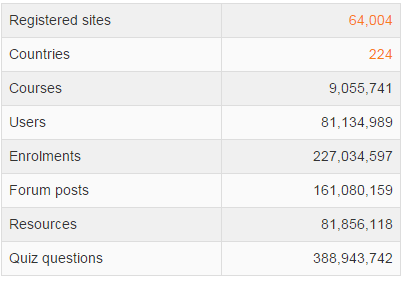
\includegraphics[width=80mm]{images/statistiky-moodle.png}
		   \end{center}
		  \caption{Počet kurzů a uživatelů ze stránek registrovaných na Moodle.org.   \cite{moodle-stats}}
		  \label{fig:moodlestats}
		\end{figure}

V listopadu roku 2010 vychází verze 2.0 a mění se systém vydávání nových verzí na šestiměsíční cykly. S novou verzí se Moodle zaměřuje také na mobilní technologie. V roce 2013 vychází plnohodnotná mobilní aplikace a také šablona vzhledu uzpůsobená zobrazení na mobilních zařízeních.

		

	\section{Vlastnosti Moodlu}
Kapitola shrnuje informace o licenční politice, komunitním rozvoji a požadavcích pro instalaci a běh aplikace. Zhodnotíme si systém s jeho výhodami i nevýhodami.
		\subsection{Licence}
Moodle není nijak závislý na licencích za počet uživatelů, přístupů či kurzů. Jedná se o nezávislý software s otevřeným zdrojovým kódem (tzv. open source) pod licencí GNU = General Public License (zkráceně GPL), která umožňuje použití pro osobní i komerční užití. Také znamená možnost jakýchkoliv úprav a vlastních doplňků a jejich další šíření, pokud souhlasíte s tím, že: \emph{budete tento zdroj poskytovat ostatním; nebudete měnit ani odstraňovat původní údaje o licencích a autorských právech, a uplatníte stejné licenční podmínky i u jakýchkoliv odvozených produktů} \cite{moodle-what-is}. 
		\subsection{Prerekvizity}
Moodle pro svůj provoz nevyžaduje specifický operační systém (je implementován v PHP) nebo databázi. Není tedy nutné platit za licence dalšího softwaru. Specifikace poslední verze\footnote{V době psaní této práce byla verze Moodle 2.9.3+.}  má následující minimální softwarovou konfiguraci pro provoz \cite{softprereq}:
\begin{itemize}
\item PHP 5.4.4
\item MariaDB 5.5.31 (a vyšší) nebo MySQL 5.5.31 (a vyšší) nebo Postgres 9.1 (a vyšší) nebo MSSQL 2008 (a vyšší) nebo Oracle 10.2 (a vyšší)
\item ostatní softwarové komponenty jsou odvozeny od operačního systému (například jako webový server může být Apache, IIS, Nginx a další) 
\end{itemize}

Mezi minimální hardwarové požadavky patří \cite{hardprereq}:

\begin{itemize}
\item dostatečně velké úložiště na materiály a zdrojové kódy Moodle; 5GB je označeno jako absolutní minimum 
\item odlišné umístění pro zálohování se stejnou nebo větší kapacitou než úložiště výše
\item minimálně 1GHz procesor, doporučuje se 2GHz dual core; skutečné nároky jsou určeny počtem uživatelů a zdrojů
\item systémová pamět minimálně 1GB; skutečné nároky jsou určeny počtem uživatelů a konfigurací stránek
\end{itemize}


		\subsection{Rozvoj}
Rozvoj Moodlu se opírá o komunitu, kterou tvoří nejen programátoři pracující na Moodle, ale také široká uživatelská základna. Komunita zastává také funkci uživatelského testování se zpětnou vazbou tvůrcům a bugreporting\footnote{hlášení chyb}. Zastává také funkci podpory, kdy si uživatelé navzájem pomáhají a radí, jak řešit problémy. Vedle komunity se během řady let vývoje Moodlu vytvořila skupina komerčních partnerů, kteří nabízejí služby spojené s Moodlem. Typicky se jedná o služby, jako je instalace Moodlu, jeho nastavení a správa, upgrade na novější verze, migrace, hosting, přizpůsobení vzhledu a funkcionality, vývoj nových rozšíření a nadstaveb a další.
		\subsection{Výhody a nevýhody}
Výše zmíněná komunita Moodlu se bezesporu řadí mezi stěžejní výhody, stejně jako sít partnerů. Mezi další výhody Moodlu patří \cite{cooch}:
\begin{itemize}
\item vícejazyčné překlady
\item relativní jednoduchost použití (tento bod jsem doplnil označením relativní, platí dle mého názoru při použití základních struktur a nastavení)
\item škálovatelnost
\item vysoká frekvence oprav a nových verzí (velké verze jsou vydávány dvakrát ročně, opravy pak na téměř denní bázi), které jsou dostupné z GITu
\item robustnost
\item bezpečnost
\item možnost instalace v cloudu
\item kompatibilita s mobilními zařízeními
\end{itemize}


Na druhou stranu má Moodle i své nevýhody. Mezi ně bychom mohli zařadit například:
\begin{itemize}
\item Náročnost na hardware - zvyšující se počet studentů úměrně zvyšuje nároky na hardware (především systémové paměti)
\item Složitá nastavení - v Moodlu můžete nastavením změnit prakticky vše od nadpisu na titulní straně až po logiku vyhodnocení známek a vytvoření webových služeb. Ačkoliv se to může jevit jako výhoda, problém je někdy v nelogickém pojmenování a vysoké závislosti mezi nastaveními. Změna jednoduchého nastavení může mít zpočátku neočekávané následky.
\item Komplikovaná změna vzhledu - Moodle ve své základní instalaci nevypadá jako moderní graficky přitažlivý systém a dostupné šablony jsou často jen variací tohoto vzhledu. Vytvoření vlastního vzhledu Moodle umožňuje, ale i pro grafika se zkušenostmi s tvorbou šablon pro Moodle to není jednoduché.
\end{itemize}

Na základě výčtu vlastností výše je zřejmé, že Moodle je skvělým nástrojem pro menší a střední organizace, střední i základní školy, či podporu části výuky na vysokých školách. Je dostupný cenově i požadavky na prostředí. Pokud jej ale chcete používat efektně a efektivně pro velké množství konkurenčně přistupujících uživatelů, nevyhnete se nákladům na kvalitní hardware a správce, často z řad komerčních partnerů a poskytovatelů služeb spojených s Moodlem. 

	\section{Kurz}
		\subsection{Rozložení}
Typickým rozložením aplikace je dvou či tří sloupcový layout, ojediněle se vyskytuje layout s jediným sloupcem. Základem každé stránky Moodle je kontejner pro vložení hlavního obsahu pro danou sekci/stránku. Při vstupu do kurzu se v něm zobrazí přehled a složení kurzu, v detailu výukového modulu se zobrazí látka daného modulu, v případě správy kurzu, modulu, Moodlu atd. je obsahem kontejneru samotný formulář s nastavením dané položky.

Boční sloupce obsahují tzv. bloky s kontextovými ovládacími prvky a doplňky (bloky si blíže představíme níže). Bloky je možné umístit do levého i pravého sloupce, čímž ovlivníme, zda výsledný vzhled bude se dvěma nebo třemi sloupci. Není-li do sloupce přidělen alespoň jeden blok, sloupec je skryt. 

U instalace bez zásahu do nastavení je při zapnutém i vypnutém režimu úprav (přepínač vypíná a zapíná ovládací prvky editace) kurz i jeho nastavení poskládáno do dvou sloupců, hlavního obsahu a kontextové nabídky pro správu kurzu a stránek.

		\subsection{Výukové moduly}
Výukovým modulem je prostor v kurzu vyplněný specifickým typem činností. Moodle definuje dvě kategorie modulů na základě toho, zda je modul interaktivní, či nikoliv. Vyžaduje-li modul aktivní přístup studenta popř. učitele, řadí se mezi tzv. činnosti. V opačném případě jde pouze o pasivní prvek nazývající se studijním materiálem.
Základní instalace Moodlu obsahuje následující výukové moduly (přehled modulů vychází z \cite{drlik} a zdrojových kódů Moodlu): 

\textbf{Činnosti}:
\begin{itemize}
\item \textbf{Anketa} - umožňuje učiteli položit otázku a definovat výběr z více odpovědí. Výsledky ankety mohou být studentům zpřístupněny poté, co odpoví, po jistém termínu nebo případně nikdy. Výsledky lze zobrazovat jmenovitě i anonymně.
\item \textbf{Balíček SCORM} - umožňuje do kurzu vložit obsah ve formátu dle specifikací SCORM a AICC. Jedná se o soubory, které jsou zabaleny podle standardu pro výukové objekty. Obsah je většinou zobrazen na několika stránkách spolu s prvkem pro navigaci mezi stránkami. Pro zobrazení obsahu existují různé možnosti - ve vyskakovacím okně, s obsahem, s navigačními tlačítky apod. Činnosti SCORM obecně zahrnují úlohy, jejichž hodnocení se zapisuje do klasifikace v kurzu.
\item \textbf{Databáze} - umožňuje vytvářet, prohlížet a prohledávat kolekci záznamů vztahujících se prakticky k libovolnému tématu. Záznamy mohou obsahovat text, obrázky, hypertextové odkazy, číselné údaje a další informace. Vzhled kolekce, jednotlivých záznamů i formuláře pro editaci lze řídit pomocí šablon. Definici struktury záznamů a jejich vzhledu lze sdílet pomocí tzv. předloh. Vyučující mohou záznamy importovat a exportovat.
\item \textbf{Dotazník} - umožňuje realizovat dotazníkové šetření. Slouží pro získání zpětné vazby od účastníků kurzu. Při návrhu dotazníku lze použít řadu typů položek včetně výběru z daných hodnot nebo volné tvořené odpovědi. Vyplněné dotazníky mohou být anonymní, je-li to žádoucí. Výsledky mohou být k dispozici i studentům, nebo pouze vyučujícím. Dotazníky na titulní stránce serveru mohou vyplňovat též nepřihlášení uživatelé.
\item \textbf{Externí nástroj} - umožňuje studentům pracovat s prostředky a činnostmi na jiných webových stránkách. Nástroj na straně poskytovatele externích služeb musí podporovat specifikaci LTI. Tvůrci kurzu mohou využívat pouze nástroje, které správce stránek přidá do seznamu externích nástrojů.
\item \textbf{Fórum} - nabízí možnost asynchronní komunikace účastníků kurzu. K dispozici je několik typů fór: běžné fórum, kde může každý začínat nové diskuse a zapojit se do stávajících; fórum, v němž může každý student začít nejvýše jednu diskusi; nebo fórum, v němž musí student nejprve sám za sebe odpovědět položené otázky před tím, než vidí odpovědi ostatních. K příspěvkům lze přikládat soubory jako přílohy. Příspěvky ve fóru je možno hodnotit, a to i ostatními studenty (vzájemné hodnocení). Hodnocení se přepočítává na výslednou známku, která může být součástí klasifikace v kurzu.
\item \textbf{Chat} - umožňuje účastníkům kurzu diskutovat na webu synchronně v reálném čase. Chatování může být jednorázovou aktivitou, nebo je lze opakovat pravidelně každý den, týden apod. Záznamy z chatu jsou uloženy a mohou být zpřístupněny všem účastníkům kurzu nebo jen vybraným uživatelům na základě nastaveného oprávnění. Chat je obzvláště užitečný v případech, kdy se účastníci kurzu nemohou setkávat tváří v tvář.
\item \textbf{Průzkum} - poskytuje řadu standardních dotazníkových nástrojů, které se osvědčily při hodnocení a stimulaci výuky v on-line prostředí. Učitel je může použít pro sběr údajů od svých studentů, které jim pomohou seznámit se se svou třídou a zamyslet se nad svým učením.

\end{itemize}
		\subsection{Bloky}
	\section{Uživatelské role a kontext}

		\begin{figure}
		  \begin{center}
		    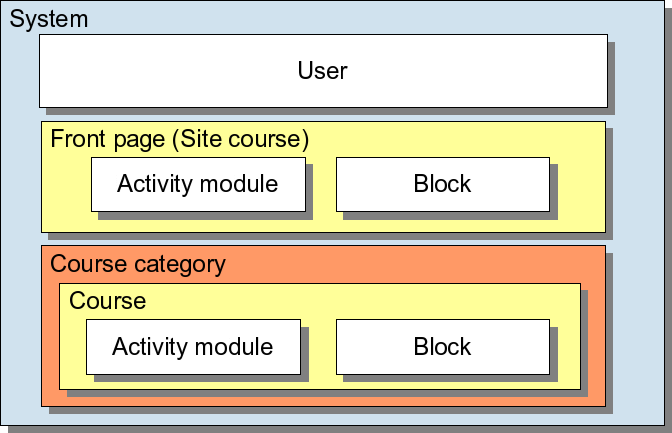
\includegraphics[width=100mm]{images/moodle-context.png}
		   \end{center}
		  \caption{Grafické zobrazení hierarchie kontextů.   \cite{moodle-context}}
		  \label{fig:moodlecontext}
		\end{figure}

	\section{Vytvoření kurzu a jeho nastaven}

		\begin{figure}
		  \begin{center}
		    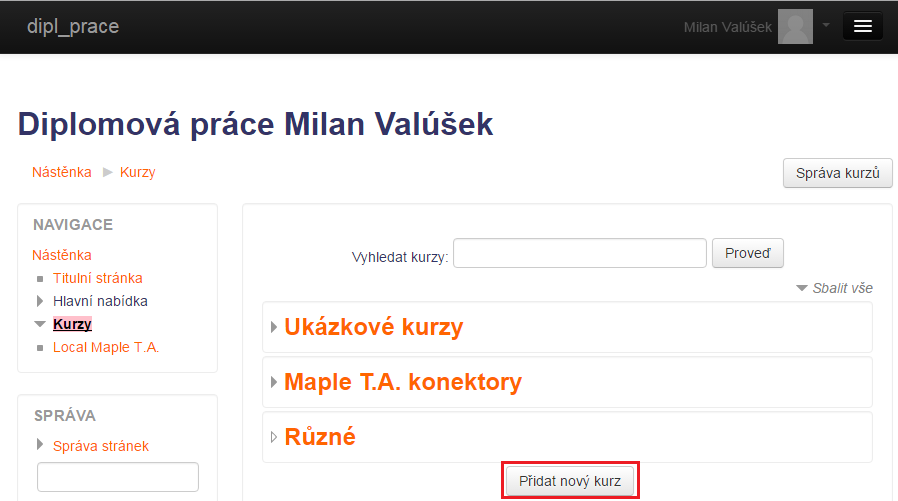
\includegraphics[width=120mm]{images/kurzy-pridani.png}
		   \end{center}
		  \caption{Náhled obrazovky s kategoriemi kurzy (uživatel s právy vytvořit kurz).  }
		  \label{fig:moodlekurzypridani}
		\end{figure}

		\begin{figure}
		  \begin{center}
		    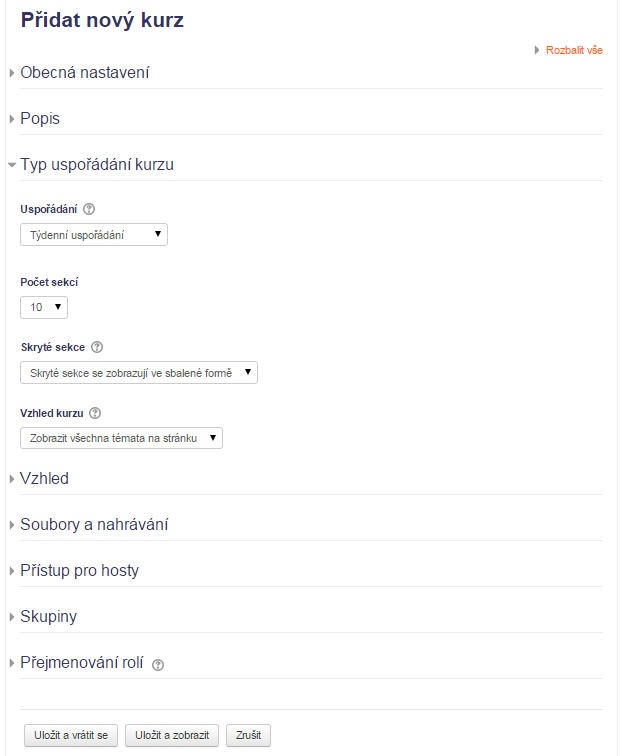
\includegraphics[width=120mm]{images/kurzy-pridani-detail.png}
		   \end{center}
		  \caption{Náhled na formulář pro přidání kurzu.}
		  \label{fig:moodlekurzypridanidetail}
		\end{figure}

\chapter{Maple T.A.}
	\section{Co je to Maple T.A.?}
		\begin{figure}
		  \begin{center}
		    
\includegraphics[width=60mm]{images/MapleTA_logo.jpg}
		   \end{center}
		  \caption{Oficiální logo Maple T.A.  \cite{maple-logo}}
		  \label{fig:maplelogo}
		\end{figure}

	\section{Licencování}
	\section{Předpoklady pro instalaci}
	\section{Základy aplikace}
		\subsection{Otázka (Question)}

		\begin{figure}
		  \begin{center}
		    
\includegraphics[width=60mm]{images/MapleTA_logo.jpg}
		   \end{center}
		  \caption{Oficiální logo Maple T.A.  \cite{maple-logo}}
		  \label{fig:maplelogo}
		\end{figure}

		\begin{figure}
		  \begin{center}
		    
\includegraphics[width=60mm]{images/MapleTA_logo.jpg}
		   \end{center}
		  \caption{Oficiální logo Maple T.A.  \cite{maple-logo}}
		  \label{fig:maplelogo}
		\end{figure}

		\begin{figure}
		  \begin{center}
		    
\includegraphics[width=60mm]{images/MapleTA_logo.jpg}
		   \end{center}
		  \caption{Oficiální logo Maple T.A.  \cite{maple-logo}}
		  \label{fig:maplelogo}
		\end{figure}

		\begin{figure}
		  \begin{center}
		    
\includegraphics[width=60mm]{images/MapleTA_logo.jpg}
		   \end{center}
		  \caption{Oficiální logo Maple T.A.  \cite{maple-logo}}
		  \label{fig:maplelogo}
		\end{figure}

		\subsection{Úkol (Assignment)}
		\subsection{Kniha hodnocení (Gradebook)}
	\section{Uživatelské role}
	\section{Vytvoření úkolu}
\chapter{Analýza}
	\section{Struktura zdrojových kódů Moodlu}
	\section{Analýza konektorů od Maple T.A.}
		\subsection{Klasický konektor}
		\subsection{LTI konektor}

\chapter{Implementace}
	\section{Webové služby Maple T.A.}
		\subsection{Kontrola připojení}
		\subsection{Vytvoření a ukončení relace}
		\subsection{Získávání a manipulace s daty}
		\subsection{Maple T.A. Launcher služby}
		\subsection{Grade pushing}
		\subsection{Monitoring}
	\section{Návrh a porovnání s ostatními konektory}
	\section{Databázový model}
	\section{Struktura modulu a její realizace}

		\begin{figure}
		  \begin{center}
		    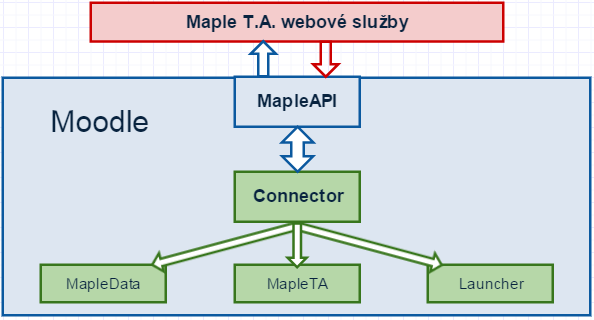
\includegraphics[width=100mm]{images/struktura_modulu.png}
		   \end{center}
		  \caption{Struktura navrhovaného modulu}
		  \label{fig:strukturamodulu}
		\end{figure}

		\begin{figure}
		  \begin{center}
		    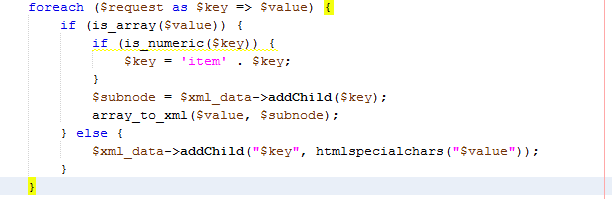
\includegraphics[width=100mm]{images/prevod_na_xml.png}
		   \end{center}
		  \caption{Algoritmus k převedí asociativního pole na XML}
		  \label{fig:prevodnaxml}
		\end{figure}

		\begin{figure}
		  \begin{center}
		    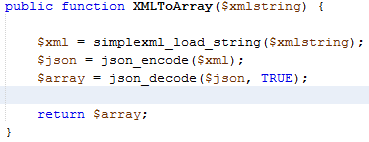
\includegraphics[width=100mm]{images/xml_na_pole.png}
		   \end{center}
		  \caption{Webové služby vrací data v podobě XML, tímto voláním se převedou na asociativní pole.}
		  \label{fig:prevodnapole}
		\end{figure}

		

	\section{Detaily implementace}
		\subsection{Vytovření nové instance}
		\begin{figure}
		  \begin{center}
		    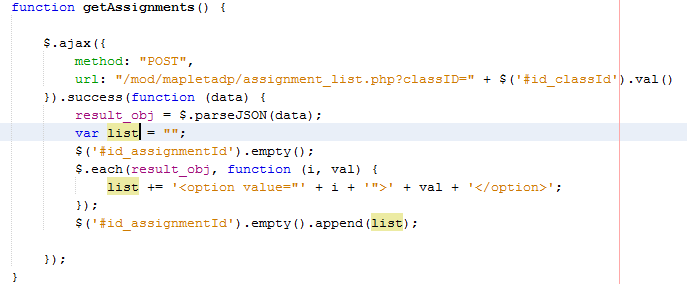
\includegraphics[width=100mm]{images/ajax-volani.png}
		   \end{center}
		  \caption{Voláním PHP za pomoci AJAXu se získávají hodnoty pro závislé pole formuláře.}
		  \label{fig:volaniajax}
		\end{figure}


		\subsection{Nová naplánovaná úloha}

		\begin{figure}
		  \begin{center}
		    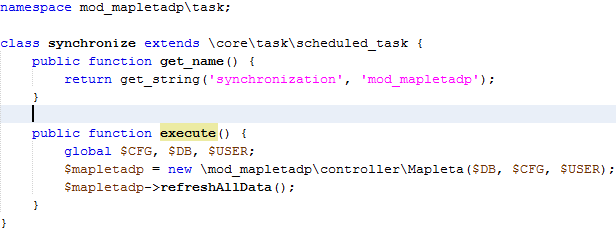
\includegraphics[width=100mm]{images/cron-trida.png}
		   \end{center}
		  \caption{Implementace třídy je využíta jako naplánovaná úloha. }
		  \label{fig:crontrida}
		\end{figure}

		\begin{figure}
		  \begin{center}
		    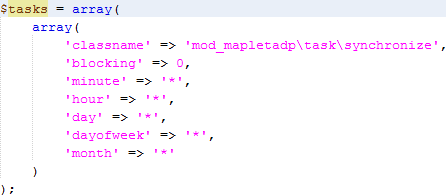
\includegraphics[width=100mm]{images/cron-registrace.png}
		   \end{center}
		  \caption{Ukázka záznamu z pole, které Moodle využivá při instalaci nové naplánované úlohy.}
		  \label{fig:cronregistrace}
		\end{figure}
\chapter{Diskuze}

\chapter{Závěr}




\printbibliography[heading=bibintoc]
\listoffigures
\listoftables




\makeatletter\thesis@blocks@clear\makeatother
\phantomsection %% Print the index and insert it into the
\addcontentsline{toc}{chapter}{\indexname} %% table of contents.

\makeatletter\thesis@blocks@clear\makeatother

\renewcommand{\theHchapter}{A\arabic{chapter}}
\appendix %% and start the appendices.

\chapter{An appendix}
Here you can insert the appendices of your thesis.

\end{document}
